%
% tschebyscheff.tex
%
% (c) 2020 Prof Dr Andreas Müller, Hochschule Rapperswil
%
\begin{frame}
\frametitle{Tschbyscheff-Stützstellen}
\begin{block}{Aufgabenstellung}
Gibt es Stützstellen derart, dass alle Extrema von $l(x)$ $\pm1$ sind?
\end{block}
\begin{center}
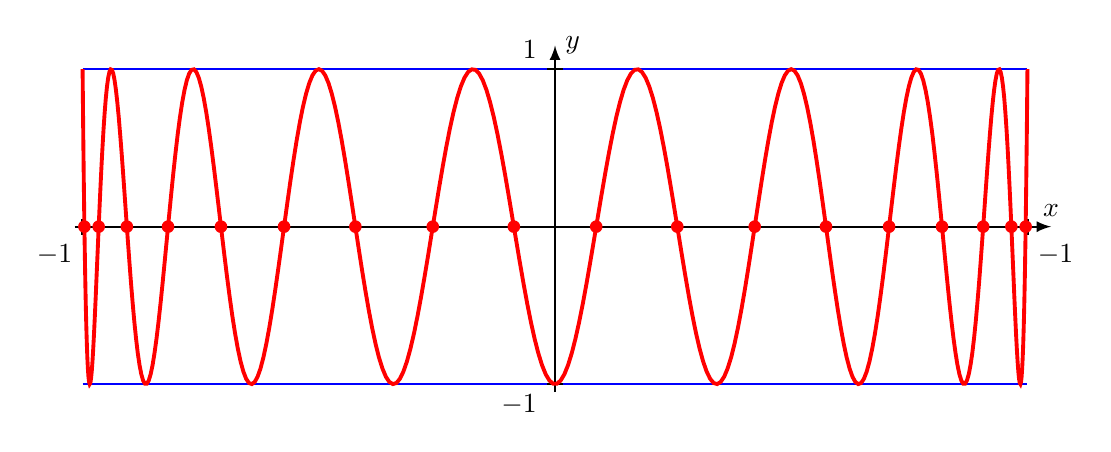
\begin{tikzpicture}[>=latex,thick]
\uncover<4->{
	\draw[color=blue,line width=0.5pt] (-6,2)--(6,2);
	\draw[color=blue,line width=0.5pt] (-6,-2)--(6,-2);
}
\draw[->] (-6.1,0)--(6.3,0) coordinate[label={$x$}];
\draw[->] (0,-2.1)--(0,2.3) coordinate[label={right:$y$}];
\draw (-0.1,-2)--(0.1,-2); \node at (-0.1,-2) [below left] {$-1$};
\draw (-0.1,2)--(0.1,2); \node at (-0.1,2) [above left] {$1$};
\draw (-6,-0.1)--(-6,0.1); \node at (-6,-0.1) [below left] {$-1$};
\draw (6,-0.1)--(6,0.1); \node at (6,-0.1) [below right] {$-1$};
\def\N{18}
\uncover<3->{
	\draw[color=red,line width=1.4pt]
		plot[domain=0:180,samples=400]
			({6*cos(\x)},{2*cos(\N*\x)});
}
\uncover<2->{
	\foreach \k in {1,...,\N}{
		\fill[color=red] ({6*cos(180*(2*\k-1)/(2*\N))},0)
			circle[radius=0.08];
}
}
\end{tikzpicture}
\end{center}
\end{frame}
